\documentclass[10pt,letterpaper,twocolumn]{article}

% This is a report artifact. It does not modify ORCHESTRA implementation,
% kernel/BPF source, tests, or benchmark scripts.
\usepackage[letterpaper,margin=0.66in,columnsep=0.24in,top=0.62in,bottom=0.66in]{geometry}
\usepackage[T1]{fontenc}
\usepackage{mathptmx}
\usepackage[scaled=0.90]{helvet}
\usepackage{microtype}
\usepackage{amsmath,amssymb}
\usepackage{booktabs}
\usepackage{tabularx}
\usepackage{array}
\usepackage{multirow}
\usepackage{makecell}
\usepackage{xcolor}
\usepackage{graphicx}
\usepackage{tikz}
\usetikzlibrary{arrows.meta,positioning,calc,fit,shapes.geometric,patterns}
\usepackage{pgfplots}
\pgfplotsset{compat=1.18}
\usepackage{titlesec}
\usepackage{enumitem}
\usepackage{fancyhdr}
\usepackage{caption}
\usepackage{balance}
\usepackage{url}
\usepackage[hidelinks]{hyperref}

\hypersetup{
  pdftitle={ORCHESTRA-OS versus Linux CFS: Evidence-Based Strengths, Weaknesses, and Field Fit},
  pdfauthor={S.W. ZAW},
  pdfsubject={Evidence-gated comparison of a sched ext prototype with Linux CFS}
}

\definecolor{navy}{HTML}{16324F}
\definecolor{cfs}{HTML}{5F6B76}
\definecolor{orch}{HTML}{0072B2}
\definecolor{good}{HTML}{009E73}
\definecolor{warn}{HTML}{D98E04}
\definecolor{bad}{HTML}{B33A3A}
\definecolor{lightblue}{HTML}{E8F2F8}
\definecolor{lightgreen}{HTML}{E8F5EF}
\definecolor{lightamber}{HTML}{FFF4D6}
\definecolor{lightred}{HTML}{F8E7E7}
\definecolor{inkgray}{HTML}{4B5563}
\definecolor{grid}{HTML}{D9E0E6}

\newcommand{\ORCH}{ORCHESTRA-OS}
\newcommand{\CFS}{Linux CFS}
\newcommand{\schedext}{\texttt{sched\_ext}}
\newcommand{\hostid}{20S1S9CY14 (ThinkPad T14 Gen 1)}
\newcommand{\AUTHOR}{S.W.\ ZAW}
\newcommand{\evidence}[1]{\textsf{\scriptsize #1}}
\newcommand{\metric}[1]{\textit{#1}}
\newcolumntype{Y}{>{\raggedright\arraybackslash}X}
\newcolumntype{R}{>{\raggedleft\arraybackslash}p{0.82in}}
\newcolumntype{C}{>{\centering\arraybackslash}p{0.72in}}

\setlength{\parindent}{1em}
\setlength{\parskip}{0pt}
\setlength{\emergencystretch}{1.5em}
\renewcommand{\baselinestretch}{0.98}
\setlist{nosep,leftmargin=*}
\captionsetup{font=footnotesize,labelfont=bf}
\titleformat{\section}{\normalfont\bfseries\scshape\small}{\thesection}{0.48em}{}
\titleformat{\subsection}{\normalfont\bfseries\itshape\footnotesize}{\thesubsection}{0.45em}{}
\titlespacing*{\section}{0pt}{1.35ex plus .3ex minus .2ex}{0.65ex}
\titlespacing*{\subsection}{0pt}{1.0ex plus .2ex minus .2ex}{0.35ex}

\pagestyle{fancy}
\fancyhf{}
\fancyhead[L]{\scriptsize EVIDENCE-GATED COMPARATIVE STUDY --- ORCHESTRA-OS}
\fancyhead[R]{\scriptsize \thepage}
\renewcommand{\headrulewidth}{0pt}
\fancypagestyle{plain}{%
  \fancyhf{}
  \fancyhead[L]{\scriptsize EVIDENCE-GATED COMPARATIVE STUDY --- ORCHESTRA-OS}
  \fancyhead[R]{\scriptsize \thepage}
  \renewcommand{\headrulewidth}{0pt}}

\tikzset{
  flowbox/.style={draw=navy,rounded corners=2pt,fill=lightblue,align=center,
    text width=1.42in,minimum height=0.43in,font=\scriptsize,inner sep=4pt},
  flowgood/.style={flowbox,draw=good,fill=lightgreen},
  flowwarn/.style={flowbox,draw=warn,fill=lightamber},
  flowbad/.style={flowbox,draw=bad,fill=lightred},
  flowarrow/.style={-{Latex[length=2mm]},draw=inkgray,line width=0.7pt}
}

\begin{document}

\twocolumn[
\begin{center}
  {\Large\bfseries\sffamily ORCHESTRA-OS versus Linux CFS:\par}
  \vspace{0.15em}
  {\Large\bfseries\sffamily Evidence-Based Strengths, Weaknesses, and Field Fit\par}
  \vspace{0.45em}
  {\normalsize Evidence synthesis for the target-matched sched\_ext prototype\par}
  \vspace{0.12em}
  {\footnotesize \AUTHOR\quad |\quad ORCHESTRA-OS Research and Validation\quad |\quad 1 September 2026\par}
\end{center}
\vspace{0.28em}
\begin{minipage}{0.965\textwidth}
\noindent\textbf{Abstract---}This validation report determines where the current ORCHESTRA-OS scheduling prototype is stronger than the Linux default CFS path, where it is weaker, and where its use is justified by evidence. The study combines the pre-kernel simulation study, the author-controlled real-machine validation archive, and the later ownership-gated bare-metal evidence tables preserved in the repository. The test host is Kali GNU/Linux Rolling x86\_64 on \hostid, running Linux \texttt{7.0.12+kali-amd64}. The comparison is claim-bounded: a simulation result is not a hardware result, a successful BPF attach is not task ownership, and an elapsed-time difference is not a causal scheduler benefit without workload and action evidence.

The strongest measured capability is selective foreground protection. In a held-out 20-pair experiment, four ImageMagick foreground resizes completed 74.24\% faster with ORCHESTRA while eight explicitly deferrable bzip2 workers received a 10-ms-per-second service budget. All 20 pairs won, all 160 foreground outputs verified, exact task ownership passed in every ORCHESTRA phase, and effective THROTTLE deferrals occurred in every phase. The corresponding background CPU service fell 97.69\%; therefore the result is service reallocation, not free total acceleration. A five-pair fixed-log experiment also favored ORCHESTRA, but CFS reached 96--97\,$^\circ$C and the result is thermally confounded and exploratory.

The negative control is equally important. In three matched fixed-work repetitions, ORCHESTRA was 1.58--2.05$\times$ slower than CFS for pure CPU work at 1--8 workers. The mixed CPU/I/O rows were 0.86--0.94$\times$ CFS time, but the sample is small and does not establish general superiority. The prototype additionally demonstrates bounded action, ownership, clean unload, stress/soak, userspace integrity, and same-node migration evidence, while kernel HMAC authentication, predictor convergence, memory stress, cross-node NUMA, distributed scheduling, and deployment readiness remain outside the validated evidence envelope.

\vspace{0.16em}\noindent\textbf{Conclusion---}The evidence supports \ORCH{} as an opt-in controller for known latency-sensitive foreground work coexisting with known deferrable background work. CFS remains the stronger default for general-purpose and pure CPU execution on this host.\par
\vspace{0.18em}\noindent\textbf{Index Terms---}Operating-system scheduling, sched\_ext, eBPF, CFS, foreground isolation, service budgeting, real-machine experimentation, evidence-based validation.
\end{minipage}
\vspace{0.3em}
\hrulefill\quad$\diamond$\quad\hrulefill
\vspace{0.22em}
]

\section{Research Question and Claim Discipline}

The practical question is not whether one scheduler can win one benchmark. It is:

\begin{quote}\small
Which observable workload shape makes ORCHESTRA's explicit signal, ownership, and action machinery useful relative to CFS, what cost does that policy impose, and which claimed capabilities remain outside the evidence?
\end{quote}

The study follows the authority order in the repository: the architectural research paper, the author-controlled real-machine validation archive, repository design and validation records, and the preserved raw result tables. The original research paper is explicitly a pre-kernel simulation study~\cite{simpaper}; its simulated coordination and prediction values are used as design evidence, not as Linux measurements. The real-machine validation report is treated as a prior evidence synthesis~\cite{valpaper}. The current repository revision and later bare-metal campaign are identified in the provenance package accompanying this report~\cite{repo}.

The evidence ladder is deliberately strict. We use \evidence{SIMULATED} for the pre-kernel study, \evidence{USERSPACE-VALIDATED} for API and control-plane checks without kernel ownership, \evidence{KERNEL-PROTOTYPED} for target-matched build/attach and source contracts, and \evidence{EXPERIMENTALLY-VALIDATED (BOUNDED)} only when repeated real-machine observations satisfy the stated ownership, correctness, and recovery gates. We never use the word ``better'' without naming whether it means lower foreground latency, stronger policy control, lower overhead, or a different safety property.

\begin{figure*}[t]
\centering
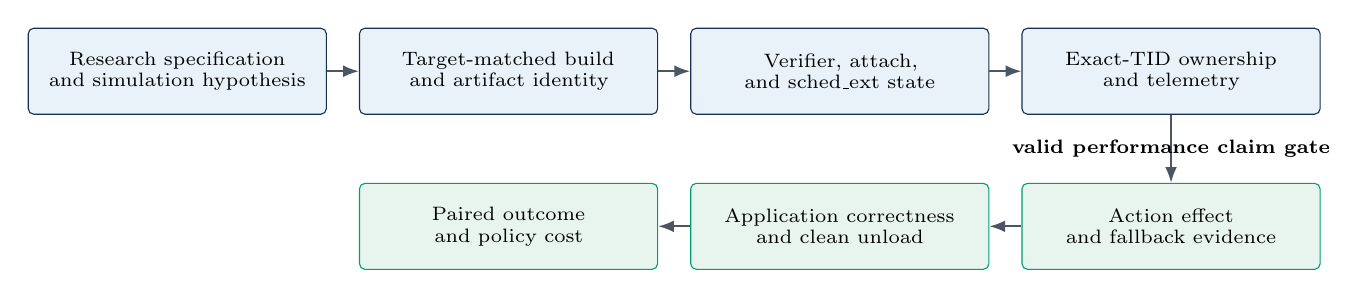
\begin{tikzpicture}[node distance=0.14in and 0.16in]
  \node[flowbox,text width=1.38in] (spec) {Research specification\\and simulation hypothesis};
  \node[flowbox,text width=1.38in,right=of spec] (build) {Target-matched build\\and artifact identity};
  \node[flowbox,text width=1.38in,right=of build] (attach) {Verifier, attach,\\and sched\_ext state};
  \node[flowbox,text width=1.38in,right=of attach] (own) {Exact-TID ownership\\and telemetry};
  \node[flowgood,text width=1.38in,below=0.34in of own] (act) {Action effect\\and fallback evidence};
  \node[flowgood,text width=1.38in,left=of act] (correct) {Application correctness\\and clean unload};
  \node[flowgood,text width=1.38in,left=of correct] (result) {Paired outcome\\and policy cost};
  \draw[flowarrow] (spec)--(build);
  \draw[flowarrow] (build)--(attach);
  \draw[flowarrow] (attach)--(own);
  \draw[flowarrow] (own)--(act);
  \draw[flowarrow] (act)--(correct);
  \draw[flowarrow] (correct)--(result);
  \node[font=\scriptsize\bfseries,above=0.08in of act] {valid performance claim gate};
\end{tikzpicture}
\caption{The evidence chain used in this report. A timing row without the middle ownership and action gates is reported as an observation or as inconclusive, not as proof that ORCHESTRA caused the difference.}
\label{fig:evidence-chain}
\end{figure*}

\section{What ORCHESTRA Adds Relative to CFS}

The Linux default path is a general-purpose scheduler. ORCHESTRA adds a policy/control surface around a target-matched \schedext{} prototype: explicit task admission, versioned signal and policy records, bounded prediction consumption, five canonical actions, action-specific telemetry, freshness/generation gates, and a bounded controller contract. This changes the optimization target. CFS is optimized to provide general-purpose scheduling behavior with low integration complexity; ORCHESTRA is designed to express differentiated service for selected tasks.

The following distinctions are supported by source and runtime evidence, not by assuming the full architecture exists in the kernel:

\begin{table*}[t]
\centering\scriptsize
\caption{Capability comparison. ``Validated'' is always scoped to the evidence class and workload stated in the last column. A dash means that CFS has no corresponding ORCHESTRA-specific interface, not that CFS is insecure or incapable of the general property.}
\label{tab:comparison}
\begin{tabularx}{\textwidth}{p{0.16\textwidth}p{0.18\textwidth}p{0.19\textwidth}Y}
\toprule
Property & CFS baseline & ORCHESTRA prototype & Evidence-based interpretation \\
\midrule
Default general-purpose service & Strong default; no project control-plane setup & Requires target-matched build, privilege, admission, and explicit lifecycle & CFS is the safer default for ordinary workloads; ORCHESTRA is opt-in. \\
Differentiated foreground/background service & No project-level per-task service-budget experiment & Explicit RUN plus budgeted THROTTLE on exact tasks & 20/20 held-out foreground-protection pairs; background service fell 97.69\%. \\
Pure CPU completion & Lower in every matched worker count in the fixed-work table & 1.58--2.05$\times$ CFS time at 1/2/4/8 workers & Negative evidence for general CPU acceleration. \\
Mixed CPU/I/O completion & Baseline reference & 0.86--0.94$\times$ CFS time in n=3 rows & Directional observation only; no causal superiority claim. \\
Action semantics & No project-specific action bridge & RUN, YIELD, MIGRATE, THROTTLE, SLEEP with requested/effective/fallback accounting & All five bounded action paths observed in the current action matrix. \\
Integrity/freshness & No ORCHESTRA signal surface & Userspace HMAC and generation/freshness/schema checks; kernel map is local-trust & Userspace integrity validated; kernel cryptographic authentication absent. \\
Real-time interaction & Existing Linux policy machinery & Adaptive admission refusal for FIFO/RR/DEADLINE and bounded FIFO/RR coexistence probe & No hard-real-time latency or starvation guarantee. \\
Scaling & Mature general-purpose baseline & Fixed bounded ABI slots; one-node target & Cross-node NUMA and distributed scheduling untested or not implemented. \\
\bottomrule
\end{tabularx}
\end{table*}

The capability table is complemented by a parameter register. It separates
source-defined contracts, experiment-selected policy values, and host-observed
CFS knobs; the latter are useful baselines but are not semantic equivalents of
the ORCHESTRA bridge. The complete machine-readable register is included as
\texttt{data/parameter\_inventory.csv}.

\begin{table*}[t]
\centering\scriptsize
\caption{Parameter-level comparison and evidence envelope. CFS values are host observations or protocol references, not claims that the two schedulers expose identical controls.}
\label{tab:parameters}
\begin{tabularx}{\textwidth}{p{0.15\textwidth}p{0.28\textwidth}p{0.24\textwidth}Y}
\toprule
Parameter & ORCHESTRA value or contract & CFS reference & Evidence boundary \\
\midrule
Action set & Five canonical actions: RUN, SLEEP, MIGRATE, THROTTLE, YIELD; requested, accepted, dispatched, effective, and fallback states are distinct & No corresponding ORCHESTRA action bridge in the CFS protocol & ACT recorded 81/81 assertions; broad workload-level action effectiveness remains scoped. \\
Service budget & P20 background set: 10 ms per 1 s (1.0\% nominal); 4 foreground plus 8 background workers on CPUs 0--7 & Same paired CFS workload and placement without the ORCHESTRA budget contract & 20/20 wins and 97.6851\% lower background CPU ticks; this is service reallocation. \\
Ownership gate & Lifetime-stable $(\mathit{tgid},\mathit{tid},\mathit{start\_boottime\_ns})$ identity; per-task bridge; 4,096-task bound & No corresponding ORCHESTRA ownership gate in the CFS baseline & P20: 20/20; LOG5: 60/60; FW3 summarized ORCHESTRA rows: ownership=yes. \\
Signal image & 128-byte canonical payload plus 32-byte HMAC-SHA256 tag; 160 bytes total; fixed-point scale 1,000; maximum age 5 s & No ORCHESTRA signal image in the CFS protocol & Userspace validation: 12/12 runs, 12,000 publications, 27,161 verified reads; kernel map remains local-trust. \\
Version safety & Signal schema 1, state schema 2, kernel ABI 8, control ABI 10; generation-stamped two-slot publication with no reuse & No corresponding ORCHESTRA generation-stamped bridge in CFS & Duplicate, stale, and invalid local checks are retained; this is not kernel HMAC validation. \\
Runtime guardrails & Slice minimum 0.1 ms, run default 5 ms, run maximum 100 ms, throttle maximum 1 s, sleep maximum 5 s, expiry/lease maximum 60 s & Host snapshot: CFS base slice 2.8 ms, migration cost 0.5 ms, migration batch 32 & Source-defined bounds and bounded action paths are evidenced; tail-latency cost is not closed. \\
Coordination & 10-ms default window; 2-ms mass-switch window; mass-switch threshold 8; $Q=(S_1S_2S_3S_4)^{1/4}$ & No valid $Q_{\mathrm{CFS}}$ mapping is defined & Bounded records and the corrected metric contract exist; broad cross-system $Q$ statistics are not claimed. \\
Controller & 100-ms default update period; 30-ms minimum hold; 200-ms cooldown and evaluation; 11 named actuators & No ORCHESTRA outer-controller surface in the CFS baseline & State and telemetry exist; full actuator causality and rollback response remain open. \\
Policy geometry & State v2: 30 states, 5 actions, 150 Q cells, 1,200 bytes per worker; directive threshold 0.82 & CFS does not use this ORCHESTRA policy table & Userspace mechanics are validated; hardware policy generalization is not established. \\
Safety and soak & FIFO/RR/DEADLINE adaptive admission refused; 3 x 600-s CPU/I/O/mixed phases; clean unload & Native Linux policy machinery remains the comparison baseline & FIFO/RR coexistence passed; DEADLINE launch was EPERM-blocked; no hard-RT guarantee. \\
Scope & 4 physical / 8 logical CPUs, one NUMA node, Linux \texttt{7.0.12+kali-amd64}; target-matched BTF and artifacts & Same host and kernel, with no BPF attach/build requirement & Same-node movement is evidenced; cross-node NUMA, distributed scheduling, and portability remain open. \\
\bottomrule
\end{tabularx}
\end{table*}

\subsection{The strongest parameter is service differentiation}

The principal strength is not a universally lower dispatch cost. It is a programmable service contract: keep a known foreground set runnable and deliberately constrain a known deferrable set. This is precisely the structure in the strongest experiment. CFS ran both groups under its default policy; ORCHESTRA ran the foreground group and charged the background group against a fixed budget. The measured foreground benefit is therefore meaningful for an interactive or urgent stage only if the operator accepts delayed background completion.

The architecture also has strong evidence hygiene. The live action matrix distinguishes a directive being requested from it being accepted, dispatched, effective, or sent to fallback. A legal MIGRATE request reached the requested and actual CPU fields; an illegal target fell back to RUN without incrementing the MIGRATE acceptance/dispatched counters. SLEEP and THROTTLE showed deferred/released state transitions, and every attached phase returned to \texttt{sched\_ext=disabled}.

\subsection{The simulated design corrections remain useful, but are not hardware results}

The simulation study found that the original three-factor coordination index could score a synchronized stampede as perfect. It added temporal stability $S_4$ and used the geometric mean:
\begin{equation}
  Q(t) = \bigl(S_1(t)S_2(t)S_3(t)S_4(t)\bigr)^{1/4}.
\end{equation}
The same study found a controller--target mismatch, a reward/directive contradiction, a state discretization ceiling, an exploration ceiling, missing local causal credit, and an online-adaptive Kalman filter whose MSE was about seven times a fixed smoother. Those findings are valuable design warnings for the prototype. They do not establish that the same parameter values or failures occur on the target kernel.

\begin{figure}[t]
\centering
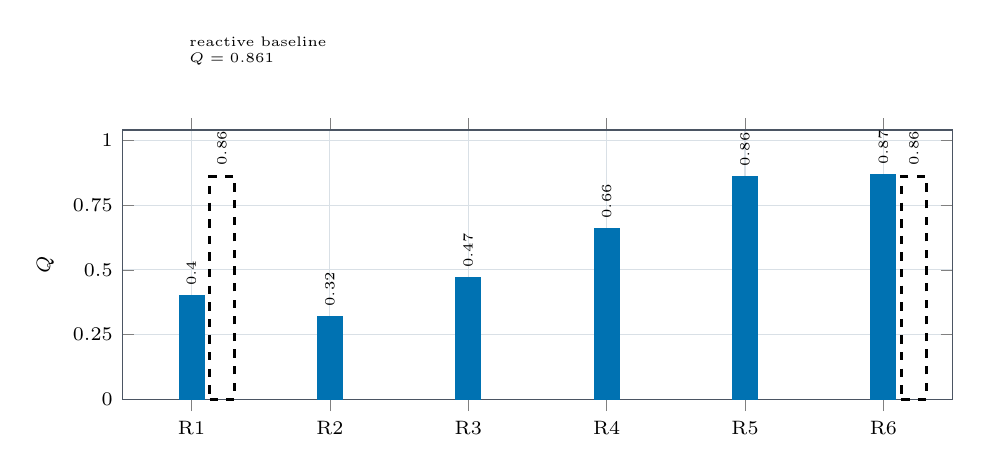
\begin{tikzpicture}
\begin{axis}[
  width=\columnwidth,
  height=5.0cm,
  ybar,
  bar width=9pt,
  symbolic x coords={R1,R2,R3,R4,R5,R6},
  xtick=data,
  ymin=0, ymax=1.04,
  ylabel={$Q$},
  ytick={0,0.25,0.5,0.75,1.0},
  grid=major,
  major grid style={draw=grid},
  axis line style={draw=inkgray},
  tick label style={font=\scriptsize},
  label style={font=\scriptsize},
  nodes near coords,
  every node near coord/.append style={font=\tiny,rotate=90,anchor=west},
  clip=false,
]
\addplot[fill=orch,draw=orch] coordinates {(R1,0.40) (R2,0.32) (R3,0.47) (R4,0.66) (R5,0.86) (R6,0.868)};
\addplot[black,dashed,very thick,forget plot] coordinates {(R1,0.861) (R6,0.861)};
\end{axis}
\node[font=\tiny,align=left,text width=1.25in] at (2.44,4.42) {reactive baseline\\$Q=0.861$};
\end{tikzpicture}
\caption{Simulation-only coordination progression from the research paper. R1--R4 use the historical raw-product/pre-$S_4$ conventions and are not magnitude-comparable with the corrected geometric-mean R5--R6 values. This plot is design evidence, not a CFS result.}
\label{fig:simulation-q}
\end{figure}

\section{Experimental Platform and Protocols}

\subsection{Platform}

The target is Kali GNU/Linux Rolling x86\_64 on \hostid. The recorded CPU is an Intel Core i5-10310U with 4 physical cores and 8 logical CPUs, one NUMA node, and approximately 31 GiB RAM. The kernel is Linux \texttt{7.0.12+kali-amd64}. The repository revision audited for the runtime campaign is \texttt{94664aeb001d8b3552245aedfd78254fbb5f13b8}; the worktree was dirty, so the campaign records the distinction between committed and uncommitted state. The exact target-matched build generated BTF from the running kernel and passed the verifier/attach gate. The final scheduler state was disabled and unrelated BPF state was preserved.

This report is a synthesis of the completed campaign archive; it does not
impute fresh heavy-run values. Tool, thermal, topology, and storage boundaries
recorded during testing remain part of the interpretation.

\subsection{Comparison protocols}

Three complementary protocols are used:

\begin{enumerate}
  \item \textbf{Fixed work.} The repository's fixed-work helper was run with identical worker counts and collection logic. Three CFS and three ownership-proven ORCHESTRA repetitions were summarized for CPU work at 1, 2, 4, and 8 workers and mixed CPU/I/O work at 1, 2, and 4 workers. The primary measure is completion time.
  \item \textbf{Foreground protection.} Twenty counterbalanced, held-out pairs used four foreground ImageMagick resizes and eight single-threaded bzip2 background workers. ORCHESTRA assigned foreground RUN and background a 10-ms-per-second THROTTLE budget. Foreground output dimensions, byte counts, and pixel signatures were checked; ownership and effective deferral were required.
  \item \textbf{Real-log candidate.} Five counterbalanced pairs used four fixed boot-journal transforms and eight gzip archive streams. The input was 104,353 JSON records. Exact foreground output identity, 12-task ownership, deferral/release telemetry, and unload were recorded. Because the CFS phases reached a near-critical thermal state, this is exploratory rather than confirmation evidence.
\end{enumerate}

For a timing ratio $r=T_{\mathrm{ORCH}}/T_{\mathrm{CFS}}$, $r>1$ means the prototype took longer. For a reduction percentage $d$, we use $d=100(1-T_{\mathrm{ORCH}}/T_{\mathrm{CFS}})$ unless the metric is explicitly background service. For the 20-pair study, the descriptive paired 95\% $t$ interval is reported without turning it into a universal population inference.

\section{Results: Fixed-Work Comparison}

Table~\ref{tab:fixed-work} and Fig.~\ref{fig:fixed-ratio} are the clearest direct comparison with CFS. Exact ORCHESTRA task ownership was positive for every summarized row. The pure CPU result is consistently unfavorable to ORCHESTRA: the ratio ranges from 1.58 at one worker to 2.05 at four workers. This is not a failure of correctness; it is evidence that the added control path, action accounting, and prototype implementation cost more than CFS for this small fixed CPU helper.

Mixed work is directionally different. ORCHESTRA's mean completion was 14.35\% lower at one worker, 5.90\% lower at two, and 10.00\% lower at four. The rows have only three repetitions, and the measurement protocol records accepted/dispatched/running ownership while some workers may exit before the final effective snapshot. We therefore call this a descriptive exploratory observation, not a general mixed-work advantage.

\begin{table}[t]
\centering\scriptsize
\caption{Matched fixed-work means from three repetitions. Values are milliseconds; SD is sample standard deviation.}
\label{tab:fixed-work}
\begin{tabular}{llrrrr}
\toprule
Work & Workers & CFS mean & CFS SD & ORCH mean & ORCH/CFS \\
\midrule
CPU & 1 & 208.67 & 1.53 & 330.00 & 1.58$\times$ \\
CPU & 2 & 208.00 & 1.73 & 418.67 & 2.01$\times$ \\
CPU & 4 & 225.67 & 30.60 & 461.67 & 2.05$\times$ \\
CPU & 8 & 295.00 & 75.03 & 511.00 & 1.73$\times$ \\
Mixed & 1 & 1632.33 & 286.88 & 1398.00 & 0.86$\times$ \\
Mixed & 2 & 1958.67 & 21.83 & 1843.00 & 0.94$\times$ \\
Mixed & 4 & 1955.00 & 27.84 & 1759.67 & 0.90$\times$ \\
\bottomrule
\end{tabular}
\end{table}

\begin{figure}[t]
\centering
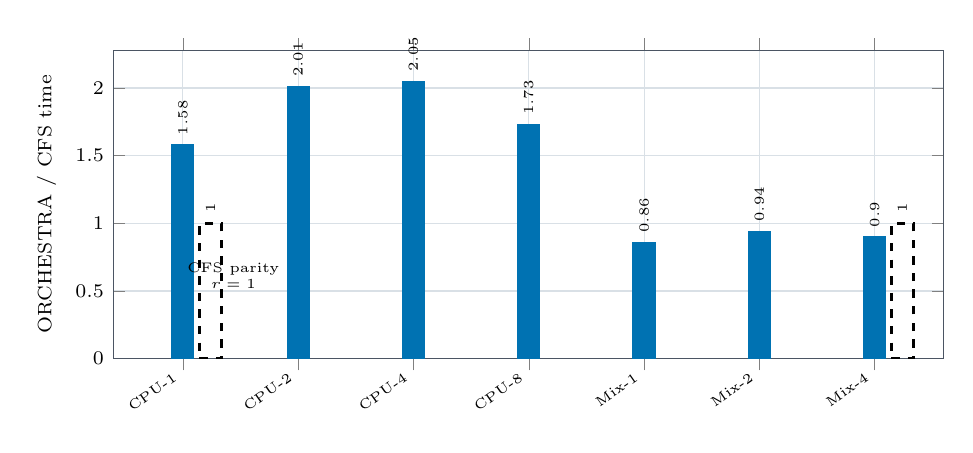
\begin{tikzpicture}
\begin{axis}[
  width=\columnwidth,
  height=5.5cm,
  ybar,
  bar width=8pt,
  symbolic x coords={C1,C2,C4,C8,M1,M2,M4},
  xtick=data,
  xticklabels={CPU-1,CPU-2,CPU-4,CPU-8,Mix-1,Mix-2,Mix-4},
  x tick label style={font=\tiny,rotate=35,anchor=east},
  ymin=0, ymax=2.28,
  ylabel={ORCHESTRA / CFS time},
  ytick={0,0.5,1,1.5,2},
  grid=major,
  major grid style={draw=grid},
  axis line style={draw=inkgray},
  tick label style={font=\scriptsize},
  label style={font=\scriptsize},
  nodes near coords,
  every node near coord/.append style={font=\tiny,rotate=90,anchor=west},
]
\addplot[fill=orch,draw=orch] coordinates {(C1,1.58) (C2,2.01) (C4,2.05) (C8,1.73) (M1,0.86) (M2,0.94) (M4,0.90)};
\addplot[black,dashed,very thick,forget plot] coordinates {(C1,1) (M4,1)};
\end{axis}
\node[font=\tiny,align=center] at (1.52,1.05) {CFS parity\\$r=1$};
\end{tikzpicture}
\caption{Fixed-work completion ratio. The CPU bars are a reproducible negative control for a universal speedup claim. Mixed bars are exploratory and should not be separated from their small sample and ownership-snapshot limitations.}
\label{fig:fixed-ratio}
\end{figure}

\section{Results: The Strongest Supported Use Case}

\subsection{Foreground protection by explicit service reallocation}

The 20-pair experiment is the strongest evidence in the package because it satisfies the full proof chain: fixed inputs, counterbalanced order, identical worker shape, exact task ownership, effective THROTTLE telemetry, application correctness, and clean unload. CFS and ORCHESTRA phases all exited zero. All 40 foreground outputs verified, including 160 individual output checks. The 20 ORCHESTRA phases all passed ownership and effective deferral, with 24--32 observed deferrals per phase.

The CFS foreground mean was 7,987.8 ms; ORCHESTRA was 2,036.6 ms. The mean reduction was 74.2405\%, with a descriptive paired 95\% $t$ interval of [72.7217\%, 75.7592\%] reduction and 20/20 ORCHESTRA wins. The median reduction was 73.7549\%. These values are strong evidence for the exact service-policy experiment, not for all work on the host.

The policy cost is visible in the same rows: mean background service fell from 4,872.85 CPU ticks under CFS to 112.80 under ORCHESTRA, a 97.6851\% reduction. Background processes remained alive at the foreground endpoint. The correct interpretation is therefore ``foreground protection against deferrable work,'' not ``the same total workload became 74\% faster.''

\begin{figure}[t]
\centering
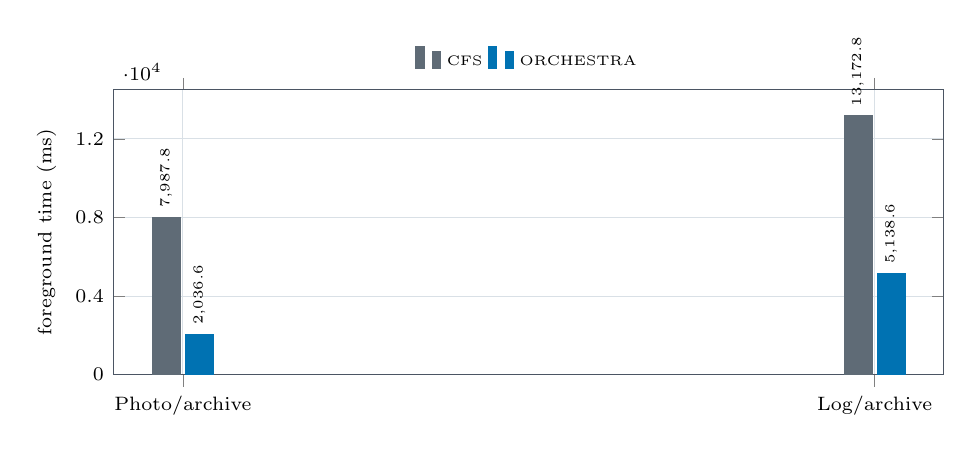
\begin{tikzpicture}
\begin{axis}[
  width=\columnwidth,
  height=5.2cm,
  ybar,
  bar width=10pt,
  symbolic x coords={Photo,Logs},
  xtick=data,
  xticklabels={Photo/archive,Log/archive},
  x tick label style={font=\scriptsize,align=center},
  ymin=0, ymax=14500,
  ylabel={foreground time (ms)},
  ytick={0,4000,8000,12000},
  grid=major,
  major grid style={draw=grid},
  axis line style={draw=inkgray},
  tick label style={font=\scriptsize},
  label style={font=\scriptsize},
  legend style={font=\tiny,at={(0.5,1.03)},anchor=south,legend columns=2,draw=none},
  nodes near coords,
  every node near coord/.append style={font=\tiny,rotate=90,anchor=west},
]
\addplot[fill=cfs,draw=cfs] coordinates {(Photo,7987.8) (Logs,13172.8)};
\addplot[fill=orch,draw=orch] coordinates {(Photo,2036.6) (Logs,5138.6)};
\legend{CFS,ORCHESTRA}
\end{axis}
\end{tikzpicture}
\caption{Foreground means for the two service-differentiation experiments. The photo result is the 20-pair confirmation; the log result is exploratory because of thermal confounding and a diagnosed transition-accounting risk.}
\label{fig:foreground-means}
\end{figure}

\begin{figure}[t]
\centering
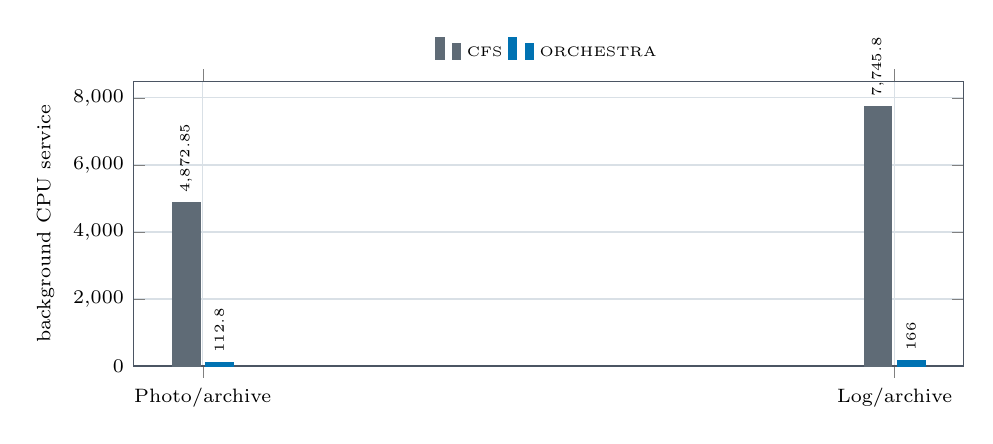
\begin{tikzpicture}
\begin{axis}[
  width=\columnwidth,
  height=5.2cm,
  ybar,
  bar width=10pt,
  symbolic x coords={Photo,Logs},
  xtick=data,
  xticklabels={Photo/archive,Log/archive},
  x tick label style={font=\scriptsize,align=center},
  ymin=0, ymax=8500,
  ylabel={background CPU service},
  ytick={0,2000,4000,6000,8000},
  grid=major,
  major grid style={draw=grid},
  axis line style={draw=inkgray},
  tick label style={font=\scriptsize},
  label style={font=\scriptsize},
  legend style={font=\tiny,at={(0.5,1.03)},anchor=south,legend columns=2,draw=none},
  nodes near coords,
  every node near coord/.append style={font=\tiny,rotate=90,anchor=west},
]
\addplot[fill=cfs,draw=cfs] coordinates {(Photo,4872.85) (Logs,7745.8)};
\addplot[fill=orch,draw=orch] coordinates {(Photo,112.8) (Logs,166.0)};
\legend{CFS,ORCHESTRA}
\end{axis}
\end{tikzpicture}
\caption{The cost side of the same result. ORCHESTRA protected foreground work by reducing background service by 97.69\% in the photo experiment and 97.86\% in the controlled log experiment.}
\label{fig:service-cost}
\end{figure}

\subsection{Real-log candidate: promising, but not a second confirmation}

The controlled log protocol used an author-controlled boot-journal fixture with 104,353 records and 133,520,770 bytes. Four foreground \texttt{jq} transforms and eight background \texttt{gzip} streams were admitted by exact task identity. ORCHESTRA won all five pairs: mean foreground time was 5,138.6 ms versus 13,172.8 ms for CFS, a 60.4678\% paired reduction. All 40 foreground outputs matched the expected transform; all 60 task-phase ownership gates passed; 675 THROTTLE events were accepted, with 248 deferrals and 208 releases; and the background service reduction was 97.8568\%.

The limitation is material. The five CFS phases measured 96--97\,$^\circ$C against the reported 100\,$^\circ$C critical point, and package-throttle counters increased. ORCHESTRA phases were cooler because the background set was strongly constrained. That may be part of the policy effect, but it also conditions the comparison. The log result is consequently \evidence{EXPLORATORY-THERMALLY-CONFOUNDED}; it identifies log/telemetry transformation as the strongest next field to validate, not as a second product guarantee.

\section{Runtime Functionality and Implementation Maturity}

The target-matched object built against the running kernel's BTF and passed verifier attach. The action matrix recorded 81/81 assertions. Selected observations are shown in Table~\ref{tab:actions}; the full matrix is included as \texttt{data/runtime\_action\_matrix.csv}.

\begin{table}[t]
\centering\scriptsize
\caption{Bounded runtime action evidence. Counts are live deltas from the action matrix, not application-wide rates.}
\label{tab:actions}
\begin{tabular}{p{0.20\columnwidth}p{0.25\columnwidth}p{0.39\columnwidth}}
\toprule
Action & Observed evidence & Interpretation \\
\midrule
RUN & dispatch 31; running 34; effective 34 & Owned RUN path observed. \\
YIELD & dispatch 45; effective 44; peer progress 32 & Queue-tail relinquish behavior observed. \\
MIGRATE & accepted 28; dispatched 28; effective 27; actual CPU 1 & Legal target movement observed; illegal target fell back to RUN. \\
SLEEP & acc./def./rel. = 1/1/1 & One-shot defer and forward progress observed. \\
THROTTLE & immediate 2/1; rollover 3/2; two-task 4/2 deferrals/releases & Generation, budget, and release accounting passed the tested matrix. \\
Unload & final state disabled & Loader-scoped lifecycle cleanup passed. \\
\bottomrule
\end{tabular}
\end{table}

The implementation matrix is more informative than a single maturity label. The five actions, local signal contract, generation/freshness checks, policy banks, controller state, RT admission boundary, and target-matched loader are implemented to different degrees. The predictor consumes bounded records but hardware convergence is not tested. The coordination contract includes $S_1$--$S_4$ and geometric-mean $Q$, with limited live windows but no broad population study. The distributed tier is absent.

\begin{table*}[t]
\centering\scriptsize
\caption{Implementation matrix used to bound claims.}
\label{tab:maturity}
\begin{tabularx}{\textwidth}{p{0.18\textwidth}p{0.16\textwidth}p{0.20\textwidth}Y}
\toprule
Component & Evidence class & Strong point & Boundary/weakness \\
\midrule
Target-matched sched\_ext scheduler, bridge, loader & \evidence{KERNEL-PROTOTYPED} & BTF-matched build, verifier attach, exact schema, scoped unload & Kernel/API-family dependence; broad portability and deployment readiness are open. \\
Five canonical actions & \evidence{EXP. BOUNDED} & Requested, accepted, dispatched, effective, and fallback outcomes are separated & Broad workload effectiveness, fairness, and long-run action interactions remain unvalidated. \\
Signal and policy contracts & \evidence{USERSPACE / KERNEL} & Generation, freshness, schema, identity, two-bank publication, bounded fallback & Kernel transport is local-trust; no kernel HMAC verifier. \\
Prediction & \evidence{USERSPACE-VALIDATED} & Bounded record consumption, confidence, expiry, observed-state fallback & No real-hardware convergence or online learning benefit. \\
Coordination $S_1$--$S_4$, $Q$ & \evidence{KERNEL / BOUNDED LIVE} & Corrected temporal-stability-aware definition is represented and limited windows are exposed & No broad population statistics; no valid fabricated $Q_{\mathrm{CFS}}$. \\
Controller & \evidence{USERSPACE / KERNEL} & Rate limits, hysteresis, saturation, rollback states, bounded actuators & Full actuator causality and rollback response are not closed. \\
RT boundary & \evidence{EXP. BOUNDED} & Adaptive path refused FIFO/RR/DEADLINE; FIFO/RR normal-task coexistence probe passed & No hard-real-time latency, starvation, or priority-inversion guarantee. \\
NUMA and distributed & \evidence{ONE NODE / ABSENT} & Same-node migration evidence on the available one-node host & Cross-node NUMA and distributed scheduling cannot be claimed. \\
\bottomrule
\end{tabularx}
\end{table*}

\section{Weaknesses, Bottlenecks, and Negative Controls}

\subsection{Pure CPU overhead is the clearest weakness}

The fixed CPU helper exposes the prototype's main disadvantage: the added policy and telemetry machinery does not pay for itself when the workload has no deferrable class to protect. At 4 workers, ORCHESTRA took 461.67 ms versus 225.67 ms under CFS. At 8 workers, it took 511.00 ms versus 295.00 ms. This is exactly the case in which the default CFS path should be preferred.

The result should not be explained as a universal scheduler cost. It is a small helper, a particular kernel and build, and a prototype path. Nevertheless, because the slowdown repeats at every CPU worker count in the matched table, it is strong evidence against advertising ORCHESTRA as a faster general-purpose replacement.

\subsection{Early RUN-to-THROTTLE transition can accept without deferring}

The prior field evidence reproduced a mechanism bottleneck. The initial log screen recorded five timing wins but zero THROTTLE deferrals, so those timings were not treated as action-causal evidence. When a fresh THROTTLE directive followed RUN before budget consumption, the early below-budget enqueue path could return after inserting a limited slice without synchronizing the task-state generation/action. The subsequent running callback saw a generation mismatch and returned before setting the running flag; the stopping callback therefore did not accumulate runtime, so the budget could remain below threshold and no deferral occurred. A short RUN warm-up before THROTTLE changed the controlled diagnostic from zero deferrals to 48 deferrals and 40 releases.

The later controlled-v6 protocol included the warm-up and observed 248 deferrals and 208 releases across five ORCHESTRA pairs. The diagnosis is high confidence because source control flow and timing-controlled before/after behavior agree, but this report does not claim that the underlying implementation has been repaired merely because the campaign's later matrix passed. This is a weakness to regression-test before relying on automated transitions.

\begin{figure}[t]
\centering
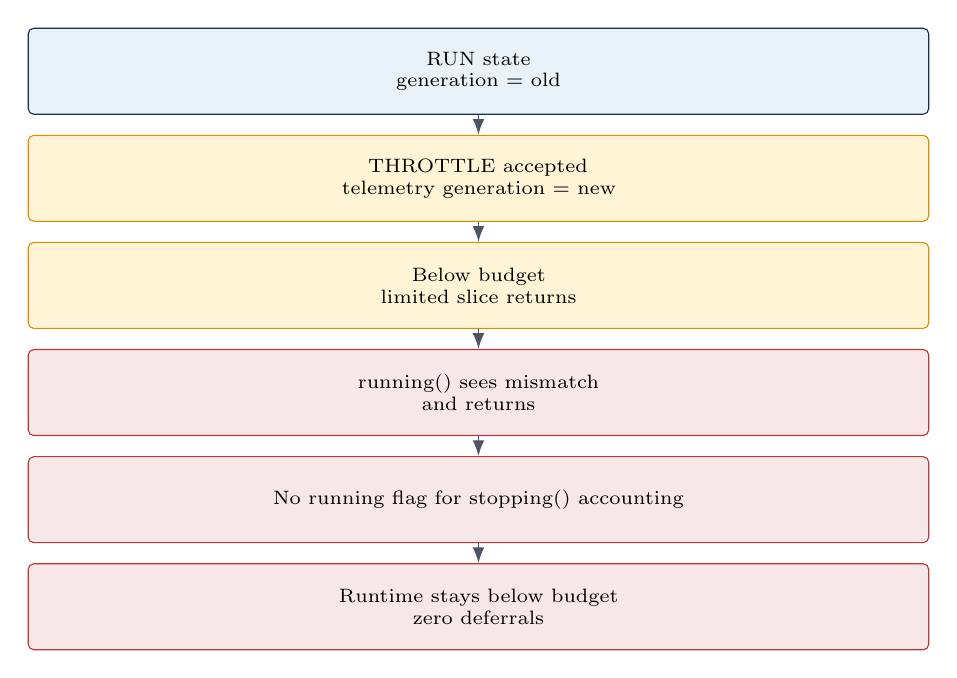
\begin{tikzpicture}[node distance=0.10in and 0.16in]
  \node[flowbox,text width=0.92\columnwidth] (run) {RUN state\\generation = old};
  \node[flowwarn,text width=0.92\columnwidth,below=of run] (throttle) {THROTTLE accepted\\telemetry generation = new};
  \node[flowwarn,text width=0.92\columnwidth,below=of throttle] (early) {Below budget\\limited slice returns};
  \node[flowbad,text width=0.92\columnwidth,below=of early] (running) {running() sees mismatch\\and returns};
  \node[flowbad,text width=0.92\columnwidth,below=of running] (runtime) {No running flag for stopping() accounting};
  \node[flowbad,text width=0.92\columnwidth,below=of runtime] (zero) {Runtime stays below budget\\zero deferrals};
  \draw[flowarrow] (run)--(throttle);
  \draw[flowarrow] (throttle)--(early);
  \draw[flowarrow] (early)--(running);
  \draw[flowarrow] (running)--(runtime);
  \draw[flowarrow] (runtime)--(zero);
\end{tikzpicture}
\caption{Source-supported diagnosis of the early RUN-to-THROTTLE accounting bottleneck. It is a preserved diagnosis and required future regression target, not a claim that an implementation repair was performed in this publication pass.}
\label{fig:throttle-bottleneck}
\end{figure}

\subsection{Multi-threaded application ownership is a product constraint}

The strongest experiment uses independent single-thread workers whose TIDs can be enumerated and admitted. The earlier standalone zstd screen won 14/20 with an interval including zero; topology inspection found multiple active TIDs even for nominally single-threaded modes. Leader-only admission therefore did not prove control of the complete work. FFmpeg was slower under the tested protocol, and SQLite mixed scheduler behavior with storage/cache/transaction effects. These are negative application screens, not universal impossibility results, but they identify a clear rule: multi-threaded applications must be admitted by complete TID enumeration or a verified group-level mechanism before timing is interpreted as an ORCHESTRA outcome.

\subsection{Security is a larger controlled surface, not an automatic advantage}

Userspace HMAC/tamper validation is strong within its scope: the focused rerun rejected explicit tamper cases with counters 201 and 42, and the documented publication microbenchmark completed 12/12 runs with 12,000 successful publications, 27,161 verified reads, and zero HMAC, invalid-frame, or stale-frame failures. Kernel-local checks rejected a \mbox{duplicate sequence} and reported stale-signal telemetry. However, the kernel map is local-trust and does not verify the HMAC. ORCHESTRA therefore adds controls for a signal/control path while also adding a root-controlled bridge, pinned maps, and loader surface. It is not intrinsically safer than CFS.

\subsection{Thermal and environment boundaries}

The log candidate reached 96--97\,$^\circ$C in CFS phases and increased package-throttle counters. The long ORCHESTRA soak completed three 600-second CPU/I/O/mixed phases, 1,800 seconds of scheduler-enabled workload time, with exact ownership, zero errors, no new critical health lines, and a maximum sampled package temperature of 87\,$^\circ$C. This is useful bounded stability evidence, not a production soak. Memory pressure remained blocked because the recorded stress harness did not provide provable child-worker ownership; the target tool inventory also did not include \texttt{scx\_simple}, \texttt{numactl}, \texttt{fio}, \texttt{iperf3}, or \texttt{perf}. These are explicit evidence boundaries, not silent exclusions.

The host has one NUMA node. The source has no multi-node backend.

\section{Where to Use ORCHESTRA}

Figure~\ref{fig:use-case} summarizes the supported field fit. The required shape is more important than the application brand:

\begin{itemize}
  \item urgent or interactive foreground work has a measurable endpoint;
  \item background work is known, enumerable, and safe to delay;
  \item the operator accepts reduced background service or delayed background completion;
  \item a target-matched privileged runtime and clean rollback path are available.
\end{itemize}

Under those conditions, candidates include interactive photo/data transformation while backup compression runs, log/telemetry parsing while older records are archived, ETL with low-priority checksum/compression workers, and maintenance tasks separated from request-serving work. These are architecture-aligned recommendations. Only the exact photo/archive protocol is experimentally validated; the log/telemetry candidate is exploratory.

For pure CPU/HPC saturation, uncontrolled database latency, internally multi-threaded media tools without full admission, memory pressure, hard real-time service, cross-node NUMA, or distributed scheduling, CFS or a purpose-built scheduler is currently the stronger choice. ORCHESTRA should not be used where delaying background completion by approximately 98\% is unacceptable.

\begin{figure*}[t]
\centering
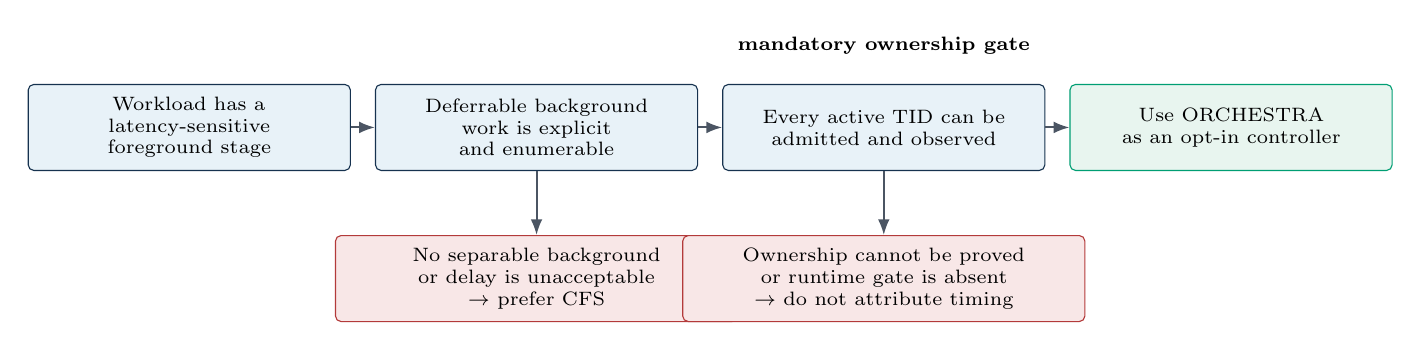
\begin{tikzpicture}[node distance=0.14in and 0.12in]
  \node[flowbox,text width=1.5in] (start) {Workload has a\\latency-sensitive foreground stage};
  \node[flowbox,right=of start,text width=1.5in] (bg) {Deferrable background\\work is explicit and enumerable};
  \node[flowbox,right=of bg,text width=1.5in] (gate) {Every active TID can be\\admitted and observed};
  \node[flowgood,right=of gate,text width=1.5in] (use) {Use ORCHESTRA\\as an opt-in controller};
  \node[flowbad,below=0.32in of bg,text width=1.9in] (cfs1) {No separable background\\or delay is unacceptable\\$\rightarrow$ prefer CFS};
  \node[flowbad,below=0.32in of gate,text width=1.9in] (cfs2) {Ownership cannot be proved\\or runtime gate is absent\\$\rightarrow$ do not attribute timing};
  \draw[flowarrow] (start)--(bg);
  \draw[flowarrow] (bg)--(gate);
  \draw[flowarrow] (gate)--(use);
  \draw[flowarrow] (bg)--(cfs1);
  \draw[flowarrow] (gate)--(cfs2);
  \node[font=\scriptsize\bfseries,above=0.10in of gate] {mandatory ownership gate};
\end{tikzpicture}
\caption{Field-fit decision rule derived from the validated workload shape. The positive result depends on an explicit foreground/background service trade-off and exact task ownership.}
\label{fig:use-case}
\end{figure*}

\section{Coordination, Prediction, and Safety Boundaries}

The original paper's most important parameter lessons are architectural rather than numerical. The corrected $Q$ must include temporal stability so synchronized mass-switching cannot look healthy. A controller must actuate the deficient submetric, not merely mutate a convenient parameter. Reward and directive boundaries must agree. State bins must align with decision thresholds. Persistent exploration imposes a compliance ceiling. Difference rewards are needed when individual actions affect population-level coordination. Finally, the failed online-adaptive Kalman result warns against assuming that more online adaptation is automatically better when process and observation noise are not identifiable.

The current kernel path represents these concepts unevenly. It exposes live bounded coordination records and controller state, but a broad $S_1$--$S_4$ population study was not completed. The correct comparison posture is not to assign a fabricated $Q_{\mathrm{CFS}}$: CFS has no corresponding ORCHESTRA signal/action index, and this report does not define a valid cross-system mapping. Similarly, the userspace HMAC result is not a kernel authentication result, and a one-node migration result is not NUMA-aware scheduling validation.

The RT evidence is bounded but useful. FIFO, RR, and DEADLINE tasks were refused adaptive admission; normal tasks coexisted, and the short FIFO/RR contention probe kept protected tasks outside the adaptive path while normal tasks remained owned. The DEADLINE contention launch was environment-blocked by EPERM. None of these observations establishes deadline latency, hard-real-time isolation, starvation freedom, or priority-inversion freedom.

\section{Statistical and Reproducibility Assessment}

The 20-pair photo experiment is the strongest quantitative result because it has 20 paired comparisons, balanced order, output verification, ownership, action, and recovery gates. Its descriptive interval and raw rows are preserved. It still represents one host, one kernel, one input family, one action policy, and one service trade-off. The five-pair log experiment is a screen under a thermal boundary, not a preregistered confirmation. The fixed-work table uses the repository’s required three repetitions for an exploratory comparison; it should be expanded to at least five repetitions with randomized order, thermal control, and complete end-state snapshots before any broad performance claim. The 47-row checklist normalizes to 38 PASS, 2 preserved FAIL, 7 BLOCKED, 0 INCONCLUSIVE, and 0 N/A; the two failures remain visible as preserved harness/attempt records.

This report's compact evidence directory includes all raw comparison rows used in the figures, the action matrix, checklist and test status, longrun table, signal microbenchmark summary, target build manifest, parameter register, diagnosis, and data dictionary. The author-controlled journal fixture is represented by its record count, byte count, expected output identity, and digest in the evidence package. The report source uses no generated numerical value that is not present in those evidence tables or the cited primary documents.

\begin{table}[t]
\centering\scriptsize
\caption{Evidence status summary.}
\label{tab:status}
\begin{tabularx}{\columnwidth}{p{0.27\columnwidth}p{0.27\columnwidth}Y}
\toprule
Area & Status & Evidence boundary \\
\midrule
Build/attach/ownership & PASS, bounded & Target-matched BPF, verifier attach, exact-TID ownership, clean unload. \\
Actions & PASS, bounded & All five observed in the action matrix; broad workload matrix pending. \\
Photo/archive protection & PASS, experimentally validated & 20/20 wins; correctness, ownership, deferral, recovery. \\
Fixed CPU & NEGATIVE, experimentally observed & ORCHESTRA 1.58--2.05$\times$ CFS time; no general speedup. \\
Mixed fixed work & EXPLORATORY & 0.86--0.94$\times$ CFS time; n=3, no causal claim. \\
Log/archive & EXPLORATORY, thermally confounded & 5/5 wins; CFS at 96--97$^\circ$C; needs cooler replication. \\
Userspace integrity & PASS, userspace only & 12/12 microbenchmark runs; kernel HMAC absent. \\
Stress/soak & PASS, bounded & 5 s, 30 s, and 30 min CPU/I/O/mixed; memory tool missing. \\
NUMA/distributed & LIMITED / NOT IMPLEMENTED & One node; same-node movement only; no distributed backend. \\
Deployment readiness & NOT ESTABLISHED & Production soak, portability, recovery breadth, and signed provenance remain open. \\
\bottomrule
\end{tabularx}
\end{table}

\section{Recommended Next Experiments}

The next work should narrow uncertainty rather than optimize for a favorable headline:

\begin{enumerate}
  \item Regression-test the early RUN-to-THROTTLE transition before-budget, after-budget, period rollover, repeated \mbox{generations}, and multiple TIDs; preserve the first failure and compare effective deferral with source-state telemetry.
  \item Repeat the log/telemetry experiment after a safe low-intensity pilot, with 20 held-out pairs, continuous thermal monitoring, and three treatments: CFS, matched cgroup CPU quota, and ORCHESTRA.
  \item Report foreground latency, background completion, total makespan, useful work, fairness, tail behavior, and energy/thermal measures together; never present foreground time alone as total speedup.
  \item Replace leader-only admission for multi-threaded tools with a proven complete-TID or group-level ownership protocol before interpreting application benchmarks.
  \item Add a target with multiple NUMA nodes and the missing benchmark tools, then validate placement, remote-memory cost, cross-node migration, memory pressure, and longer recovery behavior.
  \item Treat kernel signal HMAC, predictor convergence, full controller causality, distributed scheduling, signed provenance, and production soak as separate exit gates. None can be inferred from the present result.
\end{enumerate}

\section{Conclusion}

The evidence answers the comparison question with a conditional result. ORCHESTRA-OS is stronger than CFS when the system needs an explicit, auditable service policy that protects a known foreground set by delaying known deferrable background work. That strength is not hypothetical: the exact photo/archive protocol produced 20/20 wins, 74.24\% lower foreground completion time, 160/160 verified outputs, 20/20 ownership and effective-deferral gates, and 97.69\% lower background service.

ORCHESTRA is weaker than CFS for the tested pure CPU helper, where it took 1.58--2.05$\times$ as long. The mixed result is promising but exploratory. Its additional integrity, action, and controller surfaces improve what can be expressed and observed, but also add build, privilege, ABI, ownership, and security complexity. Kernel cryptographic authentication, predictor convergence, cross-node NUMA, distributed scheduling, broad fairness, and deployment readiness are not established.

The publishable claim is therefore precise:

\begin{samepage}
\begin{quote}\small
On Kali GNU/Linux Rolling x86\_64 running Linux \texttt{7.0.12+kali-amd64} on \hostid, the target-matched ORCHESTRA-OS prototype has a bounded, experimentally validated foreground-protection capability for explicitly deferrable background workers. It is not a generally faster replacement for CFS and is not deployment-ready.
\end{quote}
\end{samepage}

\balance
\begin{thebibliography}{9}
\footnotesize

\bibitem{simpaper}
G. Ganesan and P. Vaithiyanathan, ``ORCHESTRA-OS: Simulation-Driven Architectural Discovery and Design Principles for Predictive, Hierarchical, Signal-Coordinated Process Scheduling,'' submission draft, 6 Jul. 2026. Primary research document; all reported values are pre-kernel simulation results.

\bibitem{valpaper}
\AUTHOR, ``ORCHESTRA-OS Real-Machine Validation Archive: Field Fit and Bottleneck Evidence,'' version 2, 27 Aug. 2026. Author-controlled real-world evidence archive; source identity is recorded by SHA-256 in the accompanying provenance file.

\bibitem{repo}
\AUTHOR, ``ORCHESTRA-OS Real-World Evidence Supplement,'' companion archive, 1 Sep. 2026. It contains the reproducibility files cited in this report; complete revision and checksum information are recorded in the provenance record.

\bibitem{schedext}
Linux Kernel Documentation, ``sched\_ext: BPF extensible scheduler class,'' Linux kernel documentation, accessed 1 Sep. 2026. The target-specific attach/build boundary is also documented in the repository's kernel and installation guides.

\bibitem{woltumer}
D. H. Wolpert and K. Tumer, ``Optimal payoff functions for members of collectives,'' \textit{Advances in Complex Systems}, vol. 4, nos. 2--3, 2001.

\bibitem{kalman}
R. E. Kalman, ``A new approach to linear filtering and prediction problems,'' \textit{Journal of Basic Engineering}, vol. 82, no. 1, pp. 35--45, 1960.

\end{thebibliography}

\end{document}
